\documentclass{beamer}

\usepackage{framed}
\usepackage{graphicx}

\begin{document}
%====================================%
\begin{frame}[fragile]
\frametitle{Seaborn Workshop}
\large
\noindent \textbf{Plotting with categorical data}
\begin{itemize}
\item We previously learned how to use scatterplots and regression model fits to visualize the relationship between two variables and how it changes across levels of additional categorical variables. 
\item However, what if one of the main variables you are interested in is categorical? In this case, the scatterplot and regression model approach won’t work. There are several options, however, for visualizing such a relationship, which we will discuss in this tutorial.
\end{itemize}

\end{frame}
%===================================%
\begin{frame}[fragile]
\large
\begin{itemize}
\item It’s useful to divide seaborn’s categorical plots into two groups: those that show the full distribution of observations within each level of the categorical variable, and those that apply a statistical estimation to show a measure of central tendency and confidence interval. \item The former includes the functions \texttt{stripplot()}, boxplot(), and violinplot(), while the latter includes the functions \texttt{barplot()}, \texttt{countplot()}, and \texttt{pointplot()}. \item These functions all share a basic API for how they accept data, although each has specific parameters that control the particulars of the visualization that is applied to that data.
\end{itemize}

\end{frame}
%====================================%
\begin{frame}[fragile]
\frametitle{Seaborn Workshop}

Much like the relationship between regplot() and lmplot(), in seaborn there are both relatively low-level and relatively high-level approaches for making categorical plots. The functions named above are all low-level in that they plot onto a specific matplotlib axes. There is also the higher-level factorplot(), which combines these functions with a FacetGrid to apply a categorical plot across a grid of figure panels.

It is easiest and best to invoke these functions with a DataFrame that is in “tidy” format, although the lower-level functions also accept wide-form DataFrames or simple vectors of observations. See below for examples.
\end{frame}
%====================================%
\begin{frame}[fragile]
\frametitle{Seaborn Workshop}
\large
\begin{verbatim}
%matplotlib inline
import numpy as np
import pandas as pd
import matplotlib as mpl
import matplotlib.pyplot as plt
import seaborn as sns
sns.set(style="whitegrid", color_codes=True)
np.random.seed(sum(map(ord, "categorical")))
titanic = sns.load_dataset("titanic")
tips = sns.load_dataset("tips")
iris = sns.load_dataset("iris")
\end{verbatim}

\end{frame}
%====================================%
\section{Distributions of observations within categories}
\begin{frame}[fragile]
\frametitle{Seaborn Workshop}
Distributions of observations within categories
\begin{itemize}
\item The first set of functions shows the full distribution of the quantitative variable within each level of the categorical variable(s). 
\item These generalize some of the approaches we discussed in the chapter to the case where we want to quickly compare across several distributions.
\end{itemize}

\end{frame}
\section{Categorical scatterplots}
%====================================%
\begin{frame}[fragile]
\frametitle{Seaborn Workshop}
\large
\noindent \textbf{Categorical scatterplots}
A simple way to show the distribution of some quantitative variable across the levels of a categorical variable uses stripplot(), which generalizes a scatterplot to the case where one of the variables is categorical:

sns.stripplot(x="day", y="total_bill", data=tips);
\begin{figure}
	\centering
	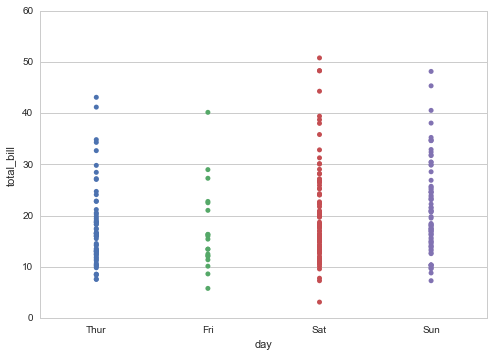
\includegraphics[width=0.7\linewidth]{images/categorical_9_0}
\end{figure}
\end{frame}
%====================================%
\begin{frame}[fragile]
\frametitle{Seaborn Workshop}
\large
It’s also possible to add a nested categorical variable with the hue paramater. Above the color and position on the categorical axis are redundent, but now each provides information about one of the two variables:
\end{frame}
%====================================%
\begin{frame}[fragile]
	\frametitle{Seaborn Workshop}
	\large
sns.stripplot(x="day", y="total_bill", hue="time", data=tips);
\begin{figure}
\centering
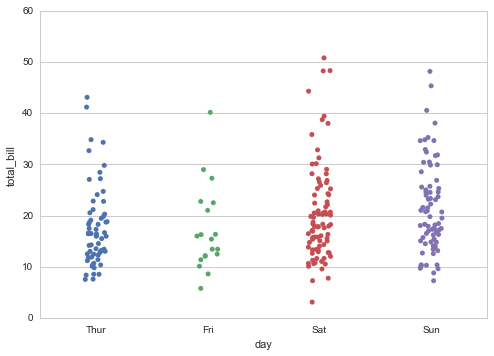
\includegraphics[width=0.7\linewidth]{images/categorical_11_0}
\end{figure}
\end{frame}
%====================================%
\begin{frame}[fragile]
	\frametitle{Seaborn Workshop}
	\large
sns.stripplot(x="size", y="total_bill", data=tips.sort("size"));
\begin{figure}
	\centering
	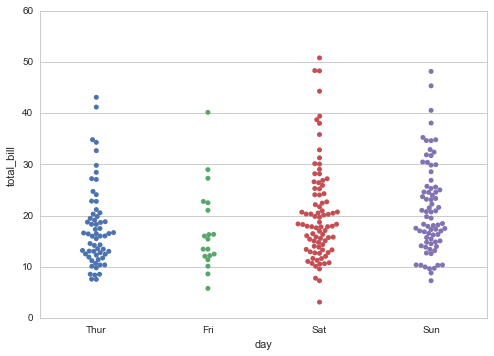
\includegraphics[width=0.7\linewidth]{images/categorical_13_0}
\end{figure}
\end{frame}
%====================================%
\begin{frame}[fragile]
\frametitle{Seaborn Workshop}
\large
With these plots, it’s often helpful to put the categorical variable on the vertical axis (this is particularly useful when the category names are relatively long or there are many categories):

sns.stripplot(x="total_bill", y="day", hue="time", data=tips);
\begin{figure}
	\centering
	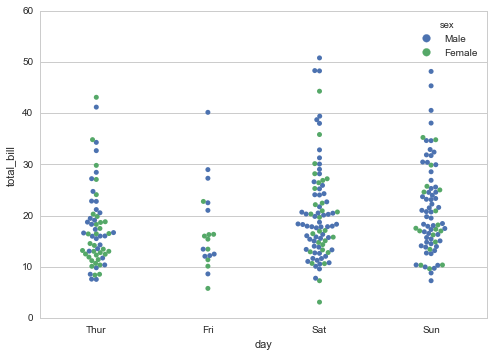
\includegraphics[width=0.7\linewidth]{images/categorical_15_0}
\end{figure}
\end{frame}
\section{Boxplots}
%====================================%
\begin{frame}[fragile]
\frametitle{Seaborn Workshop}
\large
\noindent \textbf{Boxplots}
At a certain point, the categorical scatterplot approach becomes limited in the information it can provide about the distribution of values within each category. There are several ways to summarize this information in ways that facilitate easy comparisons across the category levels.
\end{frame}
%====================================%
\begin{frame}[fragile]
The first is the familiar \texttt{boxplot()}. This kind of plot shows the three quartile values of the distribution along with extreme values. The “whiskers” extend to points that lie within 1.5 IQRs of the lower and upper quartile, and then observations that fall outside this range are displayed independently. Importantly, this means that each value in the boxplot corresponds to an actual observation in the data:
\end{frame}
%====================================%
\begin{frame}[fragile]
\begin{verbatim}
sns.boxplot(x="day", y="total_bill", hue="time", data=tips);
\end{verbatim}
\begin{figure}
	\centering
	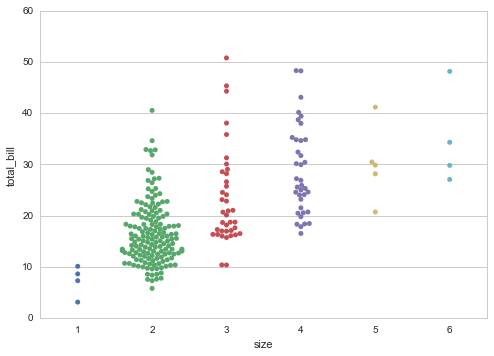
\includegraphics[width=0.7\linewidth]{images/categorical_17_0}
\end{figure}
\end{frame}
\section{Violinplots}
%====================================%
\begin{frame}[fragile]
\frametitle{Seaborn Workshop}
\large
\noindent \textbf{Violinplots}
A different approach is a violinplot(), which combines a boxplot with the kernel density estimation procedure described in the distributions tutorial
\begin{verbatim}
sns.violinplot(x="total_bill", y="day", hue="time", data=tips);
\end{verbatim}
\begin{figure}
	\centering
	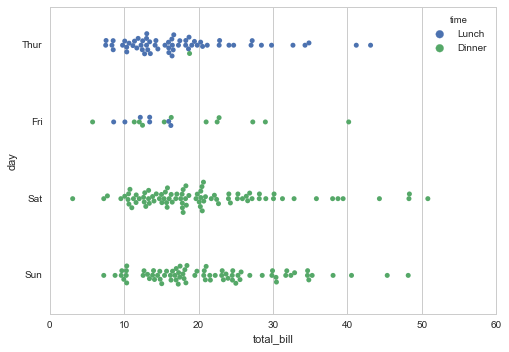
\includegraphics[width=0.7\linewidth]{images/categorical_19_0}
\end{figure}
\end{frame}
%====================================%
\begin{frame}[fragile]
\frametitle{Seaborn Workshop}
\large
This approach uses the kernel density estimate to provide a better description of the distribution of values. Additionally, the quartile and whikser values from the boxplot are shown inside the violin. Because the violinplot uses a KDE, there are some other parameters that may need tweaking, adding some complexity relative to the straightforward boxplot:
\begin{verbatim}
sns.violinplot(x="total_bill", y="day", hue="time", data=tips,
bw=.1, scale="count", scale_hue=False);
\end{verbatim}

\begin{figure}
\centering
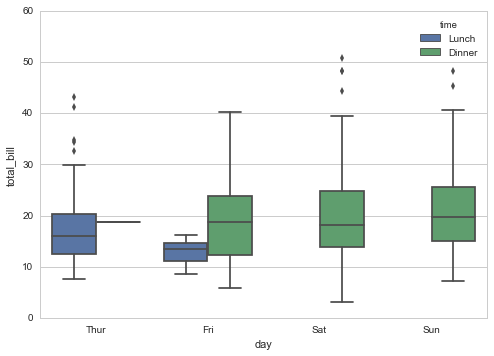
\includegraphics[width=0.7\linewidth]{images/categorical_21_0}
\end{figure}

\end{frame}
%====================================%
\begin{frame}[fragile]
\frametitle{Seaborn Workshop}
\large It’s also possible to “split” the violins when the hue parameter has only two levels, which can allow for a more efficient use of space:
\begin{verbatim}
sns.violinplot(x="day", y="total_bill", hue="sex", data=tips, split=True);
\end{verbatim}
\begin{figure}
\centering
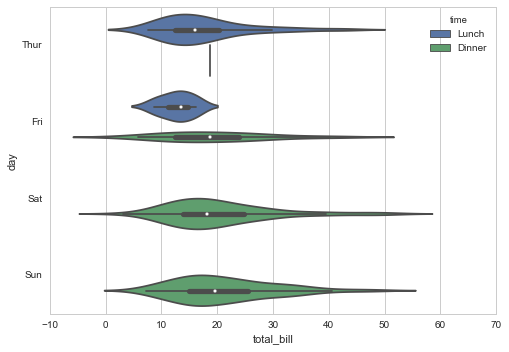
\includegraphics[width=0.7\linewidth]{images/categorical_23_0}
\caption{}
\label{fig:categorical_23_0}
\end{figure}

\end{frame}
%====================================%
\begin{frame}[fragile]
	\frametitle{Seaborn Workshop}
Finally, there are several options for the plot that is drawn on the interior of the violins, including ways to show each individual observation instead of the summary boxplot values:
\begin{verbatim}
sns.violinplot(x="day", y="total_bill", hue="sex", data=tips,
split=True, inner="stick", palette="Set3");
\end{verbatim}

\begin{figure}
	\centering
	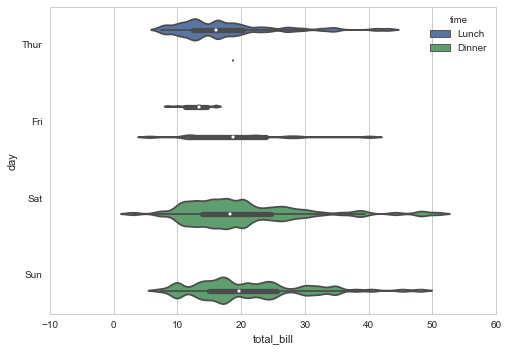
\includegraphics[width=0.7\linewidth]{images/categorical_25_0}
\end{figure}
\end{frame}
%====================================%
\begin{frame}[fragile]
	\frametitle{Seaborn Workshop}
It can also be useful to combine stripplot() with violinplot() or boxplot() to show each observation along with a summary of the distribution:
\begin{verbatim}
sns.violinplot(x="day", y="total_bill", data=tips, inner=None)
sns.stripplot(x="day", y="total_bill", data=tips, jitter=True, size=4);
\end{verbatim}
\begin{figure}
\centering
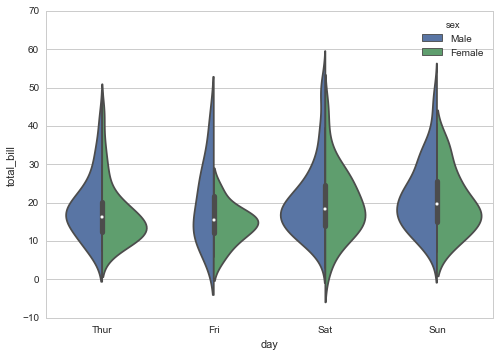
\includegraphics[width=0.7\linewidth]{images/categorical_27_0}
\end{figure}


\end{frame}
